\chapter{Particles and waves}\label{c2}
A particle is a material body whose dimensions are insignificant in comparison
with the typical dimensions of its motion. A pebble can be considered to be a
particle when one considers its projectile motion but not so when one considers
its rotation. At a more extreme level, the earth is treated like a particle when
one studies it as a part of solar system but not when we study ocean currents.
A wave, on the other hand, is a periodic disturbance. In the case of material
waves the disturbance is felt in properties of the materials. For example, the
passage of a sound waves leads to periodic compressions and rarefactions in the
material. They are detected as changes in the pressure in the case of fluids and
internal stresses in the case of solids. Electromagnetic waves do not need 
materials for their propagation and their passage is manifested in the periodic
variations in electric and magnetic field intensities at a point. Although this
distinction between particles and waves seems quite natural it is not so when 
one observes nature beyond the human senses. Newton considered light to be
particulate and it took more than two centuries to suspect that it is probably
a wave. The interference experiments of Young could be explained only by 
treating light as a wave. Maxwell predicted the existence of electromagnetic
waves and Hertz confirmed their existence. Maxwell also derived the speed of
electromagnetic waves and it was the same as the speed of light. As a result,
light was suspected to be an electromagnetic wave and was indeed shown to be so.
However, at the turn of the century other experiments were conducted whose 
outcome could not be explained by assuming that light is a wave. We will 
describe a few experiments in this chapter that demonstrate that what were
thought to be waves also behave like particles and \emph{vice versa}.

\section{Black body radiation}\label{c2s1}
Material bodies absorb and emit electromagnetic radiation. When they are in
thermal equilibrium the net absorbtion of radiation matches the net emission.
Most bodies do not absorb all radiation. They reflect or transmit it. Further,
their absorption depends on the angle of incidence. A black body is the one 
that absorbs all radiation irrespective of its wavelength and angle of 
incidence. If a blackbody is at thermal equilibrium then it should emit the
energy it absorbs. The emitted energy is called \emph{black body radiation}.
An approximately black body is a large cavity enclosed in an opaque material 
and with a small hole for radiation to get in. It is only an approximation 
because waves with wavelength greater than the hole's diameter will be 
partially reflected. Further, a finite size cavity cannot hold radiation of all
wavelengths.

Since a black body absorbs radiation of all wavelengths it also emits radiation
of all wavelengths. If $U_\lambda$ is the amount of energy in the form of 
radiation of wavelength $\lambda$ and if $V$ is it volume then 
\begin{equation}\label{c2s1e1}
u_\lambda = \frac{U_\lambda}{V}
\end{equation}
is called the `spectral energy density'. The black body radiation experiment
consists in plotting $u_\lambda$ against $\lambda$. The results of the 
experiment are shown in figure \ref{c2f1}. 
\begin{figure}
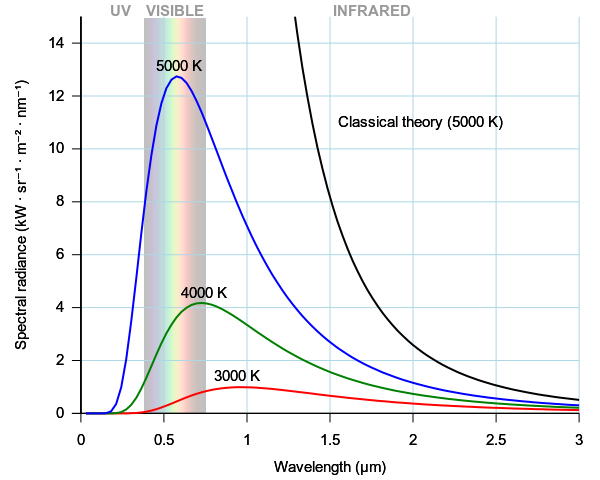
\includegraphics[scale=0.5]{Black_body}
\caption{Blackbody radiation. By Darth Kule - Own work, Public Domain, 
https://commons.wikimedia.org/w/index.php?curid=10555337}
\label{c2f1}
\end{figure}

The plot shows that as temperature
rises the dominant wavelength decreases. It agrees with the observation that
hot bodies successively appear redish to bluish to white as their temperature
increases. Lord Rayleigh and Sir James Jeans first tried to understand the
black body spectrum assuming that radiation is in the form of electromagnetic
waves. Radiation is trapped inside a black body in the form of standing waves.
If we the black body is in the form a cube of length $L$ then radiation of 
wavelength $\lambda$ will stay as a standing wave only if an integral number of
half wavelengths are accommodated in the extent $L$. If $n_x, n_y, n_z$ are the
number of half-wavelengths along the $x, y, z$ axes then
\begin{eqnarray}
n_x &=& \frac{L}{\lambda/2} = \frac{2L}{\lambda} \\
n_y &=& \frac{2L}{\lambda} \\
n_z &=& \frac{2L}{\lambda}
\end{eqnarray}
For a standing wave to form in an arbitrary direction we must have
\begin{equation}\label{c2s1e5}
n^2 = n_x^2 + n_y^2 + n_z^2 = \left(\frac{2L}{\lambda}\right)^2.
\end{equation}
In this equation we no longer require $n_x, n_y, n_z$ to be integers.
The number of waves with wavelengths between $\lambda$ and $\lambda + d\lambda$
is the number of points with positive coordinates $n_x, n_y, n_z$ in the region
between the first octant of the spheres with radii $n$ and $n + dn$. This number
is proportional to the volume of the region,
\[
\frac{1}{8} \times 4\pi n^2dn.
\]
Since there are two polarisations for each mode, the number of standing waves is
\begin{equation}\label{c2s1e6}
G(n)dn = \pi n^2 dn.
\end{equation}
From equation \eqref{c2s1e5} we have
\begin{equation}\label{c2s1e7}
n = \frac{2L}{\lambda} = \frac{2L}{c}\nu
\end{equation}
so that equation \eqref{c2s1e6} becomes
\begin{equation}\label{c2s1e8}
G(\nu)d\nu = \pi \cdot \frac{8L^3}{c^3}\nu^2d\nu.
\end{equation}
If $g(\nu)$ is the number of waves per unit volume, also called the density of
`states', then
\begin{equation}\label{c2s1e9}
g(\nu)d\nu = \frac{8\pi}{c^3}\nu^2 d\nu.
\end{equation}
Finally, in order to get the energy density, Rayleigh and Jeans used the 
classical equipartition theorem that allocates an energy of $kT/2$ to each
degree of freedom. In the case of a single standing wave, there are two degrees
of freedom so that the energy of each mode is
\begin{equation}\label{c2s1e10}
U = kT,
\end{equation}
where $k = 1.38 \time 10^{-23}$ JK${}^{-1}$ is the Boltzmann constant and $T$
is the absolute temperature. The energy density is, therefore,
\begin{equation}\label{c2s1e11}
u(\nu)d\nu = \frac{8\pi kT}{c^3}\nu^2 d\nu.
\end{equation}
One can as well express the energy density $u$ as a function of wavelength and
write
\begin{equation}\label{c2s1e12}
u(\lambda)d\lambda = \frac{8\pi kT}{\lambda^2}d\lambda.
\end{equation}
The experimentally observed energy density spectrum of a black body does not
follow these equations. In particular, when $\lambda \rightarrow 0$, or 
equivalently, $\nu \rightarrow \infty$, $u$ blows up. This feature of the 
function $u$ defined in \eqref{c2s1e10} and \eqref{c2s1e11} is called the
`ultraviolet catastrophe' and it was one of the first evidences to indicate 
that certain experiments cannot be explained by classical physics.

Max Planck's correction to this formula lay in replacing the energy given by
equation \eqref{c2s1e10} with
\begin{equation}\label{c2s1e13}
U = \frac{h\nu}{\exp(\frac{h\nu}{kT}) - 1}
\end{equation}
where $h = 6.626 \times 10^{-34}$ Js is a universal constant, now called the
Planck's constant. The expression for energy density becomes
\begin{equation}\label{c2s1e14}
u(\nu)d\nu = \frac{8\pi h\nu^3}{c^3}\frac{d\nu}{\exp(\frac{h\nu}{kT}) - 1}.
\end{equation}
This is Planck's formula for black body radiation spectrum. 

\subsection{Planck's expression for $U$}
There are many ways to derive Planck's expression in equation \eqref{c2s1e13}
for the energy of radiation. We will follow the one used originally by Planck
\cite{planck1901law}. It assumes
\begin{enumerate}
\item The relation between entropy $S$ and internal energy $U$
\begin{equation}\label{c2s1e15}
\left(\frac{\partial S}{\partial U}\right)_{V, N} = \frac{1}{T}.
\end{equation}
Here $T$ us the (absolute) temperature and $N$ is the number of particles.
\item The relation between entropy and the number of states in which a system
can be. If $\Omega$ is the number of states then
\begin{equation}\label{c2s1e16}
S = k\log\Omega
\end{equation}
where $k$ is another universal Boltzmann constant.
\item Electromagnetic energy is transferred in the units of $h\nu$, where $\nu$
is the frequency of the radiation and $h$ is a universal constant, now named 
after Planck. 
\end{enumerate}
Of these assumptions, the first one is a result in thermodynamics, known since 
the 1850s. The second one was proposed by Ludwig Boltzmann in the 1870s when he
laid the foundations of statistical mechanics while the last one was Planck's 
contribution for which he was to receive a Nobel prize in Physics in 1918.

Let the black body cavity have an energy $U_0$ at the frequency $\nu$. If there 
are $N$ modes of radiation, we want to find out the number of ways in which we 
can  distribute the energy $U$ among them. The third assumption listed above 
tells  that the energy $U$ is available as $P=U_0/(h\nu)$ packets, called quanta. 
Therefore, the problem of distribution of energy $U_0$ among the radiation modes
is the same as counting the number of ways in which $P$ quanta can be 
distributed among $N$ modes. This is an easy combinatorial problem whose 
solution is
\begin{equation}\label{c2s1e17}
\Omega = \frac{(P + N - 1)!}{P!(N - 1)!}.
\end{equation}
Usually, the number $N$ is so large that $(N - 1)! \approx N!$ so that we can
as well write \eqref{c2s1e17} as
\begin{equation}\label{c2e1e18}
\Omega = \frac{(P + N)!}{P!N!}.
\end{equation}
so that
\[
\log\Omega = \log[(P + N)!] - \log P! - \log N!.
\]
When $n$ is large, we can approximate $\log n! \approx n\log n$ (this is called
Stirling's approximation. It is quite accurate even for $n = 10$) to get
\[
\log\Omega = (P + N)\log(P + N) - P\log P - N\log N
\]
so that the entropy of the electromagnetic radiation is
\begin{eqnarray*}
S &=& k\log\Omega \\
  &=& kN\left\{\left(1 + \frac{P}{N}\right)\log(P + N) - \frac{P}{N}
      \log P - \log N\right\} \\
 &=& kN\left\{\left(1 + \frac{P}{N}\right)\log(P+N) - \frac{P}{N}
     \left(\log\frac{P}{N} + \log N\right) - \log N\right\} \\
 &=& kN\left\{\left(1 + \frac{P}{N}\right)\left(\log(P+N)-\log N\right)
     - \frac{P}{N}\log\frac{P}{N}\right\} \\
 &=& kN\left\{\left(1 + \frac{P}{N}\right)\log\left(1+\frac{P}{N}\right)
     - \frac{P}{N}\log\frac{P}{N}\right\}
\end{eqnarray*}
Since $P$ was defined as $U_0/(h\nu)$, we can write
\[
\frac{U_0}{Nh\nu} = \frac{U}{h\nu}
\]
where
\begin{equation}\label{c2s1e19}
U = \frac{U_0}{N}
\end{equation}
is the average energy per mode. We now have
\begin{equation}\label{c2s1e20}
S = kN\left\{\left(1 + \frac{U}{h\nu}\right)\log\left(1+\frac{U}{h\nu}\right)
     - \frac{U}{h\nu}\log\frac{U}{h\nu}\right\}.
\end{equation}     
From equations \eqref{c2s1e15} and \eqref{c2s1e19} one can readily show that
\begin{equation}\label{c2s1e21}
\frac{1}{T} = \frac{k}{h\nu}\left(1 + \frac{h\nu}{U}\right).
\end{equation}
This equation can be rearranged to get
\begin{equation}\label{c2s1e22}
U = \frac{h\nu}{\exp\left(\frac{h\nu}{kT}\right) - 1}
\end{equation}
which is identical with \eqref{c2s1e13}.

\subsection{Additional notes on Planck's derivation}
Planck deduced the relation $E = h\nu$ first on the basis of thermodynamic
arguments (section 2 of \cite{planck1901law}). Later on (sixth lecture in 
\cite{planck2012eight}) he gave an explanation using the mathematical 
properties of electromagnetic radiation. Chang \cite{chang2017physical} gives 
an account of Planck's theory in modern terms.

Entropy is usually introduced as a quantity measuring the disorder in a system.
The molecules of a vapour have more freedom of movement than the molecules of a
liquid. As a result we say the vapour has more entropy than a liquid. What could
entropy mean in the case of radiation? Radiation is characterised by frequency 
(or wavelength), phase and amplitude. The entropy of radiation consists in 
random fluctuations of phase and amplitude.

Although Planck introduced the idea of a quantum of energy he did not consider it
as seriously as others like Einstein, Ehrenfest and Lorentz (preface of 
\cite{planck2012eight}). In the remaining sections we will see how the idea 
turned out to have a profound and far-reaching impact on physics.

\subsection{Problem set 1}
\begin{enumerate}
\item Physics is an experimental science. We should supplement the theoretical
development of black body radiation spectrum of \eqref{c2s1e14} with an 
understanding of how it is measured. Refer to 
\url{https://physicsopenlab.org/2015/12/04/black-body-emission/} for one way to
measure the spectrum.
\item When the voltage drops an incandescent bulb gives a reddish glow. When the
voltage reaches its normal level the bulb glows bright. Can you explain the 
change in appearance based on your understanding of \eqref{c2s1e14}?
\item It is safer to use a touchless thermometer when a large number of people
have to be examined. Can you design a touchless thermometer using 
\eqref{c2s1e14}?
\item Consider the function
\begin{equation}\label{c2e1e23}
B(\nu, T) = \frac{2h\nu^3}{c^2}\frac{1}{\exp\left(\frac{h\nu}{kT}\right) - 1}.
\end{equation}
Show that it reaches an extremum at a frequency $\nu_0$ such that
\begin{equation}\label{c2e1e24}
3 + \left(\frac{h\nu_0}{kT} - 3\right)\exp\left(\frac{h\nu_0}{kT}\right) = 0.
\end{equation}
If you measure the radiation spectrum of a body using the procedure outlined
in the first problem and read the frequency $\nu_0$ at which the spectral energy 
density peaks then you can use equation \eqref{c2e1e24} to determine the 
temperature.
\item If 
\begin{equation}\label{c2e1e25}
x = \frac{h\nu_0}{kT}
\end{equation}
then equation \eqref{c2e1e24} can be written as $3 + (x - 3)e^x = 0$. You can
solve this equation using Newton's method to get $x \approx 2.821440$. Thus,
the relation between temperature of the black body and its peak frequency is
\begin{equation}\label{c2s1e26}
\frac{h\nu_0}{kT} \approx 2.821440.
\end{equation}
Using equation \eqref{c2s1e26} find the peak frequency when you measure the
radiation spectrum of
\begin{enumerate}
\item Sun whose surface temperature is approximately $6000$ K?
\item human body with temperature of $310$K? (Do you now see the usefulness
of infrared cameras?)
\end{enumerate}
On the other hand the peak frequency of the outer space is around $160$ GHz.
What is the space's temperature? (The ambient radiation in the outer space 
is called the cosmic microwave background. Can you relate it to the relativistic
Doppler effect you studied in the previous chapter?)
\end{enumerate}

\section{Photoelectric effect and X-ray generation}\label{c2s2}
When light of suitable frequency is shone on a clean metal surface, the metal
emits electrons. This is called the photoelectric effect. Experiments reported
that
\begin{itemize}
\item The electrons are emitted only if the light exceeds a certain frequency
, called the threshold frequency, which is characteristic of the metal.
\item As long as the light exceeds the threshold frequency the energy of the 
emitted electrons increases with frequency.
\item The number of electrons emitted is proportional to the intensity of light
if its frequency exceeds the threshold. If its frequency is below the threshold
the increasing intensity of light does not result in emission of electrons.
\item There is no lag between turning on the light and the emission of electrons.
\end{itemize}

None of these observations could be satisfactorily explained if one assumes that
light is a classical electromagnetic wave. A classical wave can transfer energy
to an electron in a continuous manner so that eventually the electron has enough
energy to free itself from the metal and escape.

Einstein used Planck's idea of an energy quantum to explain the experimental 
facts mentioned above (see section 8 of \cite{einstein1905heuristic}). He 
proposed that an electron in a metal has to overcome a certain energy barrier,
called the `work function' $\phi$ of the metal, before it can escape it. The
minimum frequency that the light must have for it to eject an electron is
\begin{equation}\label{c2s2e1}
h\nu_0 = \phi.
\end{equation}
If the light has a frequency $\nu > \nu_0$ then the energy $h\nu - \phi =
h(\nu - \nu_0)$ beyond the metal's work function is transferred to the
electron as its kinetic energy.

\subsection{Problem set 2}
\begin{enumerate}
\item The (first) ionization energy of an atom is the energy needed to remove
an electron from its outermost shell. Caesium atom has an ionization energy of
$3.9$ eV. However the work function of Caesium metal is only $1.9$ eV. Why are
the two different? Why is the work function lower than the ionization energy?
\item Visible light's frequency ranges from $400$ to $800$ THz. If you want 
to build a device to detect visible light using photoelectric effect, which 
metals would you use? You can consult the Wikipedia for values of work function
(\url{https://en.wikipedia.org/wiki/Work_function#Work_functions_of_elements})
of common metals. Which metals can you use to detect red light? Which ones will
suffice if you are interested only in blue and violet?
\item You have probably studied thermionic emission in the context of vacuum
tube diode. In thermionic emission electrons are ejected from a metal surface
by heating the metal. Will the thermionic work function be different from the
photoelectric work function?
\end{enumerate}

In photoelectric effect, light transfers its energy to an electron giving it
enough energy to escape from a metal. The inverse process in which a fast moving
electron is stopped by a solid releasing its energy as light is also possible.
A sharp deceleration of an electron gives rise to `bremsstrahlung', the German
word for radiation as a result of stopping (applying brakes) a charged particle.
Figure \ref{c2f1} shows the X-ray spectrum of Rhodium metal downloaded from
Wikipedia (\url{https://commons.wikimedia.org/wiki/File:TubeSpectrum.jpg#/media/
File:TubeSpectrum.jpg}).The $x$-axis has the wavelength of X-rays in picometre
($1$ pm = $10^{-12}$ m) while the $y$-axis has a quantity proportional to the
intensity of the radiation. It is observed that the spectrum is largely smooth
except for two sharp peaks and that it abruptly drops at a certain minimum
wavelength. The smooth part of the spectrum is due to bremsstrahlung while the
sharp peaks are because of transition of electrons in Rhodium atoms from higher 
energy levels to lower ones. We will understand these transitions better when we
study atomic structure in greater details in the chapters to follow.
\begin{figure}
\includegraphics[scale=0.5]{Tubespectrum}
\caption{X-ray spectrum of Rh downloaded from Wikipedia}\label{c2f2}
\end{figure}

\subsection{Problem set 3}
\begin{enumerate}
\item Figure \ref{c2f2} shows that there are no X-rays detected with a 
wavelength lesser than a certain cut-off. What does the cut-off depend on? Is 
it a characteristic of the metal or the fast moving electrons?
\item The cut-off wavelength is approximately $20$ pm. Can you estimate the 
energy of the fast moving electrons?
\item How will the cut-off wavelength change when you use faster electrons?
\item When an electron is accelerated from rest by a potential difference 
$V$ then it acquires an energy $eV$, where $e$ is the charge on the electron.
Suppose that this electron loses all its energy when it hits the metal in the
form of light of frequency $\nu_0$. Show that
\begin{equation}\label{c2s2e2}
\nu_0 = \frac{eV}{h}.
\end{equation}
Show that the corresponding wavelength is
\begin{equation}\label{c2s2e3}
\lambda_0 = \frac{hc}{eV}.
\end{equation}
The quantities $h, c$ and $e$ on the right hand side of \eqref{c2s2e3} are 
universal constants. Use their values in SI units to derive
\begin{equation}\label{c2s2e4}
\lambda_0 = \frac{1.2398 \times 10^{-6}}{V}.
\end{equation}
Equation \eqref{c2s2e4} is called Duane-Hunt law. It was derived from empirical
data before the theory of X-ray production was understood.

Does \eqref{c2s2e4} help you answer the previous two questions better?
\end{enumerate}

\section{Compton effect}\label{c2s3}
Black body radiation spectrum and photoelectric effect can be explained by
assuming that electromagnetic waves transfer energy in discrete quanta. That
perhaps makes them strange kind of waves. But there is nothing in those 
experiments to suggest that they are particles. Waves interfere, particles
collide and we can think of light as a stream of particles only when we can
make it collide with another particle. Compton's experiment involved the 
interaction of light with an electron and its results can be explained by
treating light as a stream of particles, called photons. The particles have
and energy 
\begin{equation}\label{c2s3e1}
E = h\nu,
\end{equation}
and their momentum is given by equation \eqref{c1s3e10} to be
\begin{equation}\label{c2s3e2}
p = \frac{E}{c}.
\end{equation}
Note that we still associate the term `frequency' for photons alluding to the
fact that they behave like particles and waves. Compton's experiment consisted
of shining light on electrons. If light is considered to be an electromagnetic
wave then the electron is exposed to an oscillating electric field as a result
of which it starts oscillating with the same frequency. An oscillating charge
also emits radiation so that the radiation observed after interaction with the
electron consists of the incident radiation and the emitted radiation. The
frequency of both radiations is the same although the scattered radiation is
polarised. Compton used radiation of a very high frequency in the form of X-rays
and gamma rays. He observed that the scattered radiation had a lower frequency,
or a higher wavelength. This observation could not be explained by the classical
theory. Compton, therefore, assumed that X-rays can be considered to be a 
stream of particles of energy and momentum given by equations \eqref{c2s3e1}
and \eqref{c2s3e2}. He assumed that an electron at rest has zero momentum but
it has an energy $E = m_ec^2$, $m_e$ being the mass of the electron. The
collision between the X-ray photon and a stationary electron results in the
photon getting scattered by an angle $\theta$ and the electron recoiling at 
an angle $\phi$ where the angles are measured with respect to the direction
along with the photons arrive. If we choose the $x$-axis to be along the
direction of the incident photons and if the origin is chosen to be the initial
position of the electron then $\phi$ and $\theta$ are the angles of the 
final momenta of the photon and electron with the positive $x$-axis.

Let us put expressions for initial and final momenta of the electron and the
photon. The quantities after the collision are distingushed by a prime and those
related to the electron have a subscript `e'. Thus, the initial energy and 
momenta are
\begin{eqnarray}
E &=& h\nu \label{c2s3e3} \\
\vec{p} &=& \frac{h\nu}{c}\hat{i} \label{c2s3e4} \\
E_e &=& m_ec^2 \label{c2s3e5} \\
\vec{p}_e &=& 0 \label{c2s3e6}
\end{eqnarray}
The corresponding quantities for the photon after the collision are
\begin{eqnarray}
E^\prime &=& \frac{h\nu^\prime}{c} \label{c2s3e7} \\
\pvec{p}^\prime &=& \frac{h\nu^\prime}{c}\cos\phi\hat{i} + 
                   \frac{h\nu^\prime}{c}\cos\phi\hat{j} \label{c2s3e8}
\end{eqnarray}
If $p_e^\prime$ is the magnitude of the electron's momentum after collision then
\begin{equation}\label{c2s3e9}
\pvec{p}_e^\prime = p_e^\prime\cos\theta\hat{i} + p_e^\prime\sin\theta\hat{j}
\end{equation}
and
\begin{equation}\label{c2s3e10}
E_e^\prime = \sqrt{{p_e^\prime}^2c^2 + m_e^2c^4}.
\end{equation}

Since momentum is conserved,
\begin{eqnarray}
\frac{h\nu}{c} &=& \frac{h\nu^\prime}{c}\cos\phi + p_e^\prime\cos\theta 
                   \label{c2s3e11} \\
0 &=& \frac{h\nu^\prime}{c}\sin\phi - p_e^\prime\sin\theta. \label{c2s3e12}
\end{eqnarray}
We can rearrange these as
\begin{eqnarray}
p_e^\prime c\cos\theta &=& h(\nu - \nu^\prime\cos\phi) \label{c2s3e13} \\
p_e^\prime c\sin\theta &=& h\nu^\prime\sin\phi. \label{c2s3e14}
\end{eqnarray}
Squaring and summing these
\begin{equation}\label{c2s3e15}
{p_e^\prime}^2c^2 = h^2(\nu^2 + {\nu^\prime}^2 - \nu\nu^\prime\cos\phi).
\end{equation}
Now let us consider energy conservation. After the collision, the electron
is no longer at rest. Let us assume that $T$ is its kinetic energy. It gets
it from the photon. Therefore,
\begin{equation}\label{c2s3e16}
T = h\nu - h\nu^\prime.
\end{equation}
The total energy of the electron after the collision is 
\begin{equation}\label{c2s3e17}
E_e^\prime =  T + m_ec^2.
\end{equation}
From equations \eqref{c2s3e10} and \eqref{c2s3e17},
\[
T^2 + 2m_ec^2T + m_e^2c^4 = {p_e^\prime}^2c^2 + m_e^2c^4
\]
so that
\begin{equation}\label{c2s3e18}
{p_e^\prime}^2c^2 = T^2 + 2m_ec^2T.
\end{equation}
Substituting \eqref{c2s3e16} in the above equation we get
\begin{equation}\label{c2s3e19}
{p_e^\prime}^2c^2 = h^2(\nu^2 + {\nu^\prime}^2 - 2\nu\nu^\prime) + 
                    2m_ec^2h(\nu - \nu^\prime).
\end{equation}
Finally, from equations \eqref{c2s3e15} and \eqref{c2s3e19} one get
\begin{equation}\label{c2s3e20}
\frac{m_e}{h}\left(\frac{c}{\nu^\prime} - \frac{c}{\nu}\right) = 1-\cos\phi.
\end{equation}
Since $c/\nu = \lambda$ and $c/\nu^\prime = \lambda^\prime$, we can as well
write \eqref{c2s3e20} as
\begin{equation}\label{c2s3e21}
\lambda^\prime - \lambda = \frac{h}{m_ec}(1 - \cos\phi).
\end{equation}
The expression on the right hand side of the above equation is called the
`Compton shift'. Observe that it depends on $\phi$ the angle at which one
observes the scattered photon.

\subsection{Problem set 4}
\begin{enumerate}
\item Mathematically it is clear that the Compton shift depends on the angle
of observation. Can you explain it solely on physical grounds?
\item Compton shift depends only on the angle of observation of the scattered
photon. The other terms are universal constants. In particular, the Compton
shift is independent of characteristics of the incident photon. Why did Compton
use X-rays when so many other choices of radiation were available?
\end{enumerate}

\subsection{About photons}
We used the term `photon' for the first time in this section. We used it to mean
a `light particle'. However, one should not imagine propagation of light as a
stream of particles of finite extent. Although it might have been the original
idea, the modern concept of photon is does not permit such a picture. A 
pragmatic choice, at this stage, is just to assume that light can be associated
with an energy $E = h\nu$ and a momentum $p = E/c$ and conceptally one can 
treat it as if it were a particle. To know more about why the idea of photon is
subtle and how physicists sometime get it wrong, refer to Willis Lamb's article
\cite{lamb1995anti} or a more extensive set of articles in 
\cite{roychoudhurioptics}. The same caution applies to the `phonons', the 
acoustic counterpart of photons, which we will study the specific heat of 
solids.

\section{de Broglie waves}\label{c2s4}
Experimental evidence forced Max Planck, Albert Einstein and Arthur Compton to
propose and accept that idea that electromagnetic waves show particle-like
properties. The proposal was tortuous and the acceptance reluctant. If
waves can behave like particle, might particles behave like waves? There was
no experimental evidence to suspect this possibility in 1924 when the French
physicist Louis de Broglie proposed it. It was firmly in the realm of 
speculation. However within a matter of three years the speculation was put to
rest by an experiment that demonstrated that electrons do get diffracted. In
this section, we will review de Broglie's ideas and describe the experiments
that proved them right.

We learnt in chapter \ref{c1} that photons of energy $E = h\nu$ have a momentum
\begin{equation}\label{c2s4e1}
p = \frac{E}{c} = \frac{h\nu}{c} = \frac{h}{\lambda}.
\end{equation}
de Broglie proposed that a particle with momentum $p$ has a wavelength
\begin{equation}\label{c2s4e2}
\lambda = \frac{h}{p}.
\end{equation}
Let us understand the profound implications of this mathematically innocuous
rearrangement of the terms of equation \eqref{c2s4e1}. We know that the momentum
of a particle of mass $m$ moving with a velocity $\vec{v}$ is
\begin{equation}\label{c2s4e3}
\vec{p} = \gamma m\vec{v},
\end{equation}
where 
\begin{eqnarray*}
\gamma &=& \frac{1}{\sqrt{1 - \beta^2}} \\
\vec{\beta} &=& \frac{\vec{v}}{c} 
\end{eqnarray*}
Therefore, the wavelength of the particle is
\begin{equation}\label{c2s4e4}
\lambda = \frac{h}{\gamma mv}.
\end{equation}
The energy of a body is $E = \gamma mc^2$. Therefore, its frequency is
\begin{equation}\label{c2s4e5}
\nu = \frac{E}{h} = \frac{\gamma mc^2}{h}
\end{equation}
and the velocity of its wave is
\begin{equation}\label{c2s4e6}
v_p = \nu\lambda = \frac{\gamma mc^2}{h}\frac{h}{\gamma mv} = \frac{c^2}{v}.
\end{equation}
We learnt in chapter \ref{c1} that material bodies always travel slower than
light. That is $v < c$. As a result, from equation \eqref{c2s4e6}, it is
evident that
\begin{equation}\label{c2s4e7}
v_p > c.
\end{equation}
The theory of relativity proposed that no information can travel faster than
light. So what kind of information is contained in a wave whose speed is given
by \eqref{c2s4e6}? To understand that, we need a brief interlude to refresh
our ideas about waves.

\subsection{The equation of a wave}
Any wave can be expressed with the equation
\begin{equation}\label{c2s4e8}
y = A\cos\left(2\pi\left(\frac{x}{\lambda} - \nu t\right)\right).
\end{equation}
The wave travels along the positive $x$ axis causing a displacement along the
$y$ axis. Its crest, or trough, or any other point with a fixed phase, travels
at a speed $v_p = \nu\lambda$. The subscript $p$ emphasizes that this is the
velocity of a point of a fixed phase. It is called the phase velocity. We saw
in equation \eqref{c2s4e7} that the phase velocity of de Broglie waves is
greater than the speed of light. Is there something else associated with a 
wave whose velocity matches the velocity of the particle?

To do that, we introduce the angular frequency
\begin{equation}\label{c2s4e9}
\omega = 2\pi\nu
\end{equation}
and the wave number
\begin{equation}\label{c2s4e10}
k = \frac{2\pi}{\lambda}
\end{equation}
to rewrite the equation of wave motion as
\begin{equation}\label{c2s4e11} 
y = A\cos(kx - \omega t)
\end{equation}
so that the phase velocity can also be written as
\begin{equation}\label{c2s4e12}
v_p = \frac{\omega}{k}.
\end{equation}

Now consider a superposition of two waves
\begin{eqnarray}
y_1 &=& A\cos(kx - \omega t) \label{c2s4e13} \\ 
y_2 &=& A\cos((k + \delta k)x - (\omega + \delta\omega)t). \label{c2s4e14}
\end{eqnarray}
The net displacement of any point on the $x$ axis is
\begin{equation}\label{c2s4e15}
y = y_1 + y_2 = A\left[\cos(kx-\omega t) + 
  \cos((k + \delta k)x - (\omega + \delta\omega)t)\right].
\end{equation}
Using standard trignometric identities, one can write the above equation as
\begin{equation}\label{c2s4e16}
y = 2A\cos\left[\left(k+\frac{\delta k}{2}\right)x - \left(\omega + 
\frac{\delta\omega}{2}\right)t\right]\cos\left(\frac{\delta k}{2}x - 
\frac{\delta\omega}{2} t\right).
\end{equation}
Now assume that $\delta k \ll k$ and $\delta\omega \ll \omega$ so that $k + 
\delta k/2 \approx k$ and $\omega + \delta\omega/2 \approx \omega$ and hence
\begin{equation}\label{c2s4e17}
y = 2A\cos\left(\frac{\delta k}{2}x - \frac{\delta\omega}{2}t\right)
    \cos(kx - \omega t)
\end{equation}
The superposition of the two waves \eqref{c2s4e13} and \eqref{c2s4e14} is thus
another wave with its amplitude modulated by the first cosine factor in
\eqref{c2s4e17}. The velocity of the modulation is
\begin{equation}\label{c2s4e18}
v_g = \frac{\delta\omega}{\delta k},
\end{equation}
which in the limit $\delta k \rightarrow 0, \delta\omega \rightarrow 0$ becomes
\begin{equation}\label{c2s4e19}
v_g = \frac{d\omega}{dk}.
\end{equation}
$v_g$ is called the group velocity of thewave $y$.

\subsection{Group velocity of de Broglie waves}
From equation \eqref{c2s4e4}
\begin{equation}\label{c2s4e20}
k = \frac{2\pi}{\lambda} = \frac{2\pi}{h}\gamma mv
\end{equation}
so that
\begin{equation}\label{c2s4e21}
\frac{dk}{dv} = \frac{2\pi}{h}\frac{m}{(1 - \beta^2)^{3/2}}.
\end{equation}
Likewise, from \eqref{c2s4e5}
\begin{equation}\label{c2s4e22}
\omega = 2\pi\nu = \frac{2\pi}{h}\gamma mc^2
\end{equation}
so that
\begin{equation}\label{c2s4e23}
\frac{d\omega}{dv} = \frac{2\pi}{h}\frac{mv}{(1 - \beta^2)^{3/2}}.
\end{equation}
From equations \eqref{c2s4e23} and \eqref{c2s4e21} we readily get
\begin{equation}\label{c2s4e24}
v_g = \frac{d\omega}{dk} = \frac{d\omega/dv}{dk/dv} = v.
\end{equation}
It is not the phase velocity but the group velocity of the de Broglie waves
that is physically significant. In fact, the group velocity is \emph{the}
velocity of the particle.

\subsection{Problem set 5}
\begin{enumerate}
\item Waves for which $\omega$ and $k$ have are proportional are called
non-dispersive waves. Show that for non-dispersive waves the group velocity is
identical with the phase velocity.
\item Are electromagnetic waves in vacuum dispersive or non-dispersive?
\item Derive equations \eqref{c2s4e21} and \eqref{c2s4e23}.
\item Mention the word `wave' and most people think of waves on water. Waves
in fluids are some of the most complicated waves one can come across. Read 
the article \url{https://en.wikipedia.org/wiki/Dispersion_(water_waves)} for a
glimpse of their complexity and an understanding of what dispersion means.
\item The equation
\begin{equation}\label{c2s4e25}
y = A\cos(kx + \omega t)
\end{equation}
also represents a wave. What is the difference between the waves represented
by \eqref{c2s4e25} and \eqref{c2s4e8}?
\end{enumerate}

\section{Davisson-Germer experiment}\label{c2s5}
`Light travels in a straight line' is what everyone learns first in optics. If
this were strictly true then all objects would cast a sharp shadow. If you hold
your hand in front of a light source and observe its shadow on a wall you will
observe that there is a central dark shadow of your palm is surrounded by a 
less darker outline of the palm. It happens because light rays bend as they go
past your palm. This phenomenon in which waves past a sharp edge bend is called
diffraction. Diffraction is a characteristic of waves.

Diffraction happens when light is made to pass through one or more narrow slits.
A grating is an optical instrument with a very large number of slits. It is
made by etching corrugations on a glass plate. Any regular, periodic arrangement
of a transparent material is a grating. 

Visible light is diffracted by grating made of glass. Electromagnetic waves of
much shorter wavelengths like X-rays need gratings whose `slits' are far more
closely etched. It is hard to manufacture such grating but nature provides an
alternative in the form of crystals. When X-rays are shone on a crystal the
diffracted rays form a series of intensity peaks which depend on the geometry
and symmetry of the crystal. Observing a diffraction pattern of X-rays is not
surprising. Davisson and Germer observed a diffraction pattern when they
replaced X-rays with electrons giving the first evidence in support of de
Broglie's speculation that particles have wave-like features.

Electrons being charged particles interact strongly with the crystals. As a 
result they undergo significant accelaration in the crystal. A change in their
momentum is accompanied with a change in their wavelength. It makes an analysis
of electron diffraction rather challenging. In modern times neutrons are used
in the place of electrons. They are neutral and do not interact with the crystal
as much as electrons do. They too result in a diffraction pattern further
corroborating de Broglie's hypothesis.

\subsection{Problem set 6}
\begin{enumerate}
\item The molecular weight of N$_2$ gas is $28$ g per mole. That is, $N_A$ 
number of N$_2$ molecules weigh $28$ g, where $N_A$ is the Avogadro number.
\begin{enumerate}
\item Find the mass of one N$_2$ molecule.
\item The root mean square speed of a gas molecule of mass $m$ at temperature
$T$ is
\begin{equation}
u = \sqrt{\frac{3kT}{m}}.
\end{equation}
Find the root mean square of a Nitrogen molecule at $300$ K. Hence compute its
mometum.
\item What is the de Broglie wavelength of the Nitrogen molecule? Compare it 
with the typical mean free path which is of the order of $10^{-6}$ m.
\end{enumerate}

\item A typical cricket ball weighs $160$ g and typical fast bowler gives it a
speed of $130$ kmph. What is the ball's de Broglie wavelength after it 
leaves the bowler.
\end{enumerate}

\section{Towards uncertainty relation}\label{c2s6}
We understand what waves are physically. Water waves are undulations on the
surface of water, sound waves are a succession of rarefactions and compressions
in air, electromagnetic waves are fluctuations of electric and magnetic fields
at a point. What are electrons waves? What undulates when an electron wave 
passes by?

Electron waves, or de Broglie waves in general, are represented mathematically
by a wave function $\psi$. It is a function of position $\vec{r}$ and time $t$.
In general, $\psi$ is a complex valued function. That is, for a given $\vec{r}$
and $t$, $\psi(\vec{r}, t)$ is a complex number. The quantity $|\psi|^2 = \psi
\psi^\ast$ is a real quantity. It is proportional to the probability of finding
a particle at a point $\vec{r}$ and time $t$. This statement is not accurate
because the probability of finding a particle exactly at $\vec{r}$ and exactly
at time $t$ is always zero. The correct interpretation of $\psi^2$ is that
it is the probability of finding the particle in a small volume $dV$ around
$\vec{r}$ between times $t$ and $t + dt$. 

de Broglie waves are thus waves of a function $\psi$ whose squared modulus has
is the probability density function of finding the particle in a neighbourhood
of a point and in an interval of time.

A probabilistic interpretation of $|\psi|^2$ indicates that there is never a 
certainty of finding a particle in a small enough region around a point 
$\vec{r}$. The standard deviation of $|\psi|^2$ at $\vec{r}$ is a measure of
uncertainty of finding the particle in the neighbourhood. If we restrict 
ourselves to one dimension, that is if $\psi$ is function of $x$ and $t$ then
the uncertainty of finding a particle in the neighbourhood of a point $x_0$ is
denoted by $\Delta x$. 

Armed with this understanding of $\psi$ let us consider a wave whose wavelength
is known precisely. If $\lambda$ is known then so is $k = 2\pi/\lambda$. Such
a wave looks like the one in figure \ref{c2f3}. Its squared modulus is shown in
figure \ref{c2f4}. How can one tell where the particle is? It seems like the
particle can be just about anywhere where $|\psi|^2$ is not close to zero. The
uncertainty of finding it is fairly large.
\begin{figure}
\begin{center}
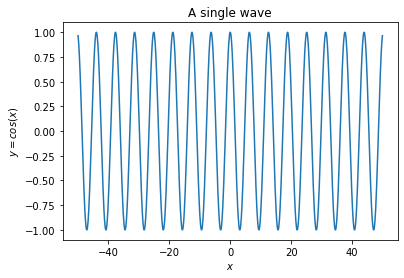
\includegraphics[scale=0.5]{one-wave}
\caption{A wave with precise $k$.}\label{c2f3}
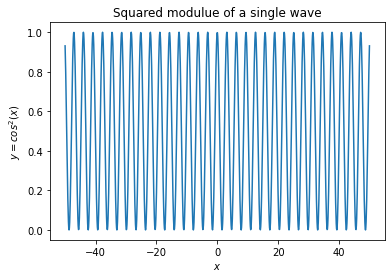
\includegraphics[scale=0.5]{one-wave-sq}
\caption{Squared modulus of a wave with precise $k$.}\label{c2f4}
\end{center}
\end{figure}
Figures \ref{c2f5} and \ref{c2f6} show a plots for a wave formed by 
superposition of two sinusoidal waves. Now we do not know the precise $k$, for 
we have mixed two of them, but we get a slightly improved localisation of the
particle.
\begin{figure}
\begin{center}
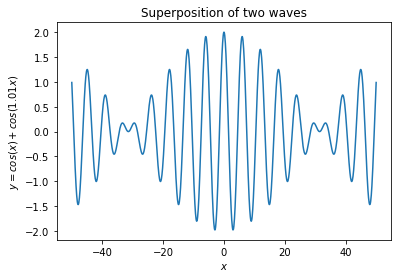
\includegraphics[scale=0.5]{two-waves}
\caption{Superposition of two cosine waves.}\label{c2f5}
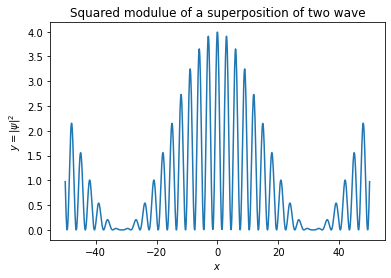
\includegraphics[scale=0.5]{two-waves-sq}
\caption{Squared modulus of superposition of waves.}\label{c2f6}
\end{center}
\end{figure}

If we repeat the exercise by mixing ten sinusoidal waves, we get the pair of
images \ref{c2f7} and \ref{c2f8}. We observe a much better knowledge of the
particle's position at the cost of losing information of $k$. We can now say
with a great confidence that the particle is likely to be in a small 
neighbourhood of the origin. 
\begin{figure}
\begin{center}
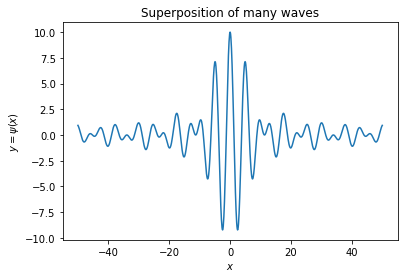
\includegraphics[scale=0.5]{ten-waves}
\caption{Superposition of ten cosine waves.}\label{c2f7}
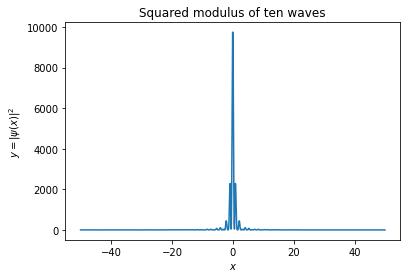
\includegraphics[scale=0.5]{ten-waves-sq}
\caption{Squared modulus of superposition of ten waves.}\label{c2f8}
\end{center}
\end{figure}

These pictures indicate that there is always a trade-off in knowing $k$ and
knowing $x$. If you think this is just the mathematical property of sinusoids
you are absolutely correct. It is indeed a mathematical property that
\begin{equation}\label{c2s6e1}
\Delta x \Delta k \ge \frac{1}{2}.
\end{equation}
Physics connects momentum with $k$ through the equation
\begin{equation}\label{c2s6e2}
p = \frac{h}{\lambda} = \frac{h}{2\pi}k
\end{equation}
so that we can write equation \eqref{c2s6e1} as
\begin{equation}\label{c2s6e3}
\Delta x \Delta p \ge \frac{h}{4\pi}.
\end{equation}
This is the celebrated `Heisenberg uncertainty relation'. It tells us that
we cannot \emph{simultaneously} know the position and momentum of a particle.
We illustrate the uncertainty relation by considering a particle in one 
dimension. As a result, its position and momentum had just one component. 
However, in general, a particle will have three position components $(x, y, z)$
and three momentum components $(p_x, p_y, p_z)$. The complete set of uncertainty
relations is
\begin{eqnarray}
\Delta x \Delta p_x &\ge& \frac{h}{4\pi} \label{c2s6e4} \\
\Delta y \Delta p_y &\ge& \frac{h}{4\pi} \label{c2s6e5} \\
\Delta z \Delta p_z &\ge& \frac{h}{4\pi}. \label{c2s6e6}
\end{eqnarray}
However,
\begin{eqnarray}
\Delta x \Delta p_y &=& 0 \label{c2s6e7} \\
\Delta x \Delta p_z &=& 0 \label{c2s6e8} \\
\Delta y \Delta p_x &=& 0 \label{c2s6e9} \\
\Delta y \Delta p_z &=& 0 \label{c2s6e10} \\
\Delta z \Delta p_x &=& 0 \label{c2s6e11} \\
\Delta z \Delta p_y &=& 0 \label{c2s6e12}
\end{eqnarray}
Equations \eqref{c2s6e7} to \eqref{c2s6e12} guarantee that one can measure the
$x$ component of a particle and $p_y$ or $p_z$ components of its momentum with
arbitrary precision. Why is $\Delta x \Delta p_x \ge h/(4\pi)$ but $\Delta x
\Delta p_y = 0$? This question cannot be answered informally using the pictures
of superposed waves and their square modulii. The answer will be partly clear
when we study quantum mechanics later in this course.

\subsection{Problem set - 6}
\begin{enumerate}
\item An atom's size is of the order of $1$ A${}^\circ$. It means that the 
uncertainty in the position of an electron in it is also of the same order.
What is the minimum uncertainty in momentum? What is the minimum uncertainty in
kinetic energy? (Assume that the electron moves at non-relativistic speed so
that its kinetic energy is $T = p^2/(2m_e)$, $m_e$ being the mass of the 
electron.
\item Energy of nucleons (protons and neutrons) is of the order of $1$ MeV.
Can you estimate the size of the nucleus using the uncertainty relation?
\end{enumerate}


